Recall the IFS \((m_1, m_2, \ldots, m_8)\) for the Minkowski Sausage \(M\) is:

\begin{align*}
    S_1((x, y)) &= \left(\frac{1}{4}x, \frac{1}{4}y\right),\\
    S_2((x, y)) &= \left(-\frac{1}{4}y + \frac{1}{4}, \frac{1}{4}x\right),\\
    S_3((x, y)) &= \left(\frac{1}{4}x + \frac{1}{4}, \frac{1}{4}y + \frac{1}{4}\right),\\
    S_4((x, y)) &= \left(\frac{1}{4}y + \frac{1}{2}, -\frac{1}{4}x + \frac{1}{4}\right),\\
    S_5((x, y)) &= \left(\frac{1}{4}y + \frac{1}{2}, -\frac{1}{4}x - \frac{1}{4}\right),\\
    S_6((x, y)) &= \left(\frac{1}{4}x + \frac{1}{2}, \frac{1}{4}y - \frac{1}{4}\right),\\
    S_7((x, y)) &= \left(-\frac{1}{4}y + \frac{3}{4}, \frac{1}{4}x - \frac{1}{4}\right),\\
    S_8((x, y)) &= \left(\frac{1}{4}x + \frac{3}{4}, \frac{1}{4}y\right).\\
\end{align*}

Notice this satisfies the OSC by considering a open square \(O\) with vertices at
\[(0, 0), (1, 0), \left(\frac{1}{2}, \frac{1}{2}\right), \left(\frac{1}{2}, -\frac{1}{2}\right),\] as shown in the following diagram.

\begin{center}
    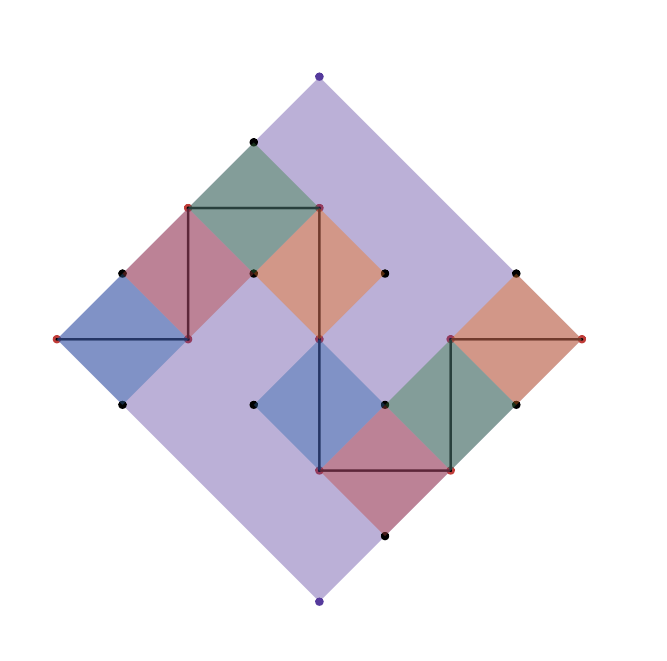
\includegraphics[scale=0.3]{solutions/section-5-0/diag-5-0-5-1.png}
\end{center}

Therefore, the dimension of \(M\), \(m\) must satisfy that
\[
8 \cdot \frac{1}{4^m} = 1 \iff m = \frac{3}{2} = 1.5,
\]
by theorem 4.1.2

Let \(M_0 = [0, 1]\) the closed interval. Let \(I_n = (i_1, i_2, \ldots, i_n)\) be a list with each \(i_k \in \{1, 2, \ldots, 8\}\), and set
\[
S_{I_n}(M_0) = S_{i_1}\left(S_{i_2}\left(\ldots\left(S_{i_n}(M_0)\right)\right)\right),
\]

Define the natural measure as
\[
\mu(S_{I_n}(M_0) \cap M) = \left(\frac{1}{4}\right)^{mn} = 8^{-n}.
\]

Let \(\mu\) be the natural measure on \(M\), the Minkowski sausage. Define
\[
\mathcal{M}_n = \{S_{I_n}(M_0) : I_n \in \{1, 2, \ldots, 8\}^n\}
\]
be the collection of all \(8^n\) scaling of size \(4^{-n}\) of the Minkowski Sausage, and let \(\{E_i\}_i \subset \mathcal{M}_n\) be a non-empty collection of those iterations of the scaling, define
\[
b_n = \min_{\{E_i\}_i \subset \mathcal{M}_n} \left\{\frac{|\bigcup_i E_i|^m}{\mu(\bigcup_i E_i)}\right\}.
\]

\textbf{Claim.} \(\h^m(M) \leq b_n\).

\textit{Proof.} We first show \(\h_\delta^m(M) \leq b_n\) for \(\h_1^m(M)\).

Since \(b_n\) is a minimum of some finite number of possibilities (subsets of the finite set \(\mathcal{M}_n\)), so there must be a collection of set \(U\) with \(\#U = k\) that gives the minimum of \(b_n\). Let \(\mathcal{U} = \bigcup_{E_i \in U} E_i\), the union of the elements in the collection \(U\).

In the case where \(\mathcal{U} = M\) is the Minkowski Sausage, then we see that this must be a cover of the Minkowski Sausage. In this case,
\[
b_n = \frac{|M|^m}{\mu(M)} \geq \frac{1^m}{1} = 1,
\]
since notice that the Minkowski Sausage contains the points \((0, 0)\) and \((1, 0)\) and they are distance of 1 apart, and noticing that \(S_{I_0} (M) = M\) so \(\mu(M) = 1\) naturally.

On the other hand, notice that \(\h_{1}^m(M) \leq 1^m = 1\) since the set containing the closed square with vertices at \((0, 0), (1, 0), \left(\frac{1}{2}, \frac{1}{2}\right)\) covers \(M\) and has diameter \(1\), and therefore from the definition, \(\h_{1}^m(M) \leq 1\) as desired. Therefore, \(\h_1^m(M) \leq 1 \leq b_n\) and satisfies the claim as desired.

Otherwise, let \(V = \mathcal{M}_n \setminus U\), all sets that are not contained in the collection \(U\). \(\# V = 8^n - k\). If for some \(S_{I_n} (M) = E_{m}' \in V\) that is not in \(U\), we scale down of these, and place it in \(V\) in the sense \(\mathcal{M}_{2n}\), the \(2n\)-th level of the construction of \(M\). If \(U\) is scaled down to \(U'\) and \(\mathcal{U}' = \bigcup_{E_i \in U} E_i\), we will see \(|\mathcal{U}'| = 4^{-n}|\mathcal{U}|\). Therefore, there will be \(8^n - k\) copies of these \(U'\)(s), one each for each element in \(\mathcal{M}_n\) that \(U\) does not hit. However this still does not cover \(M\) (since there are still missing pieces in each of parts of \(V\)), so we repeatedly create \(U''\), \(U'''\), etc.

Therefore, we cover \(M\) using 1 copy of \(\mathcal{U}\), \((8^n - k)\) copies of \(\mathcal{U}'\), \((8^n - k)^2\) copies of \(\mathcal{U}''\), and so on. Therefore,
\begin{align*}
    \h_1^m(M) &\leq \sum_{i = 0}^{+\infty} (8^n - k)^i |\mathcal{U}^{(i)}|^m\\
    &= \sum_{i = 0}^{+\infty} (8^n - k)^i (4^{-in} |\mathcal{U}|)^m\\
    &= |\mathcal{U}|^m \sum_{i = 0}^{+\infty} \left(\frac{8^n - k}{8^n}\right)i\\
    &= \frac{|\mathcal{U}|^s}{1 - \frac{8^n - k}{8^n}}\\
    &= \frac{|\mathcal{U}|^s}{\frac{k}{8^n}}\\
    &= \frac{|\mathcal{U}|^s}{\mu(\mathcal{U})}\\
    &= b_n,
\end{align*}
the first inequality sign arising due to definition, the second due to what we just show, the third by sum properties, the fourth by geometric series, the fifth by trivial algebra, the sixth by the definition of \(\mu(\mathcal{U})\) and that \(\mathcal{U}\) being the union of \(k\) copies of the \(n\)th iteration of the Minkowski Sausage which only share at most points which has dimension \(0\) so zero \(m\)-dimension measure, the seventh equal sign simply by definition of \(b_n\).

Now, we move on to \(\delta < 1\), and there must exist some \(t \in \N\) such that \(4^{-t} < \delta\). Therefore, instead with starting the cover \(U\) states in the previous part, we simply start with \(8^t\) copies of \(U\) scaled down by \(4^{-t}\), one at each level \(t\) iteration of \(M\). Then we simply preform the same process for each scaled down copies of \(U\), and at each stage we get \(8^n\) extra copies of \(U^{(n)}\), with a diameter scaled by \(4^{-n}\), and therefore
\begin{align*}
    \h_{\delta}^m(M) &\leq 8^t \sum_{i = 0}^{+\infty} (8^n - k)^i (4^{-t} |\mathcal{U}^{(n)}|)^m\\
    &= 8^t \cdot 4^{-t \cdot \frac{3}{2}} \sum_{i = 0}^{+\infty} (8^n - k)^i (|\mathcal{U}^{(n)}|)^s\\
    &= \sum_{i = 0}^{+\infty} (8^n - k)^i (|\mathcal{U}^{(n)}|)^s\\
    &= b_n
\end{align*}
similar to earlier. The largest size we used in this cover is \(4^{-t} < \delta\) is valid. Therefore, if we take the limit \(\delta \to \infty\), we will have
\[
\h^m(M) \leq b_n.
\]

Now consider the bounds of \(b_n\) when \(n = 2\). Consider the following diagram of the second iteration of \(M\), i.e., \(\mathcal{M}_2\).

\begin{center}
    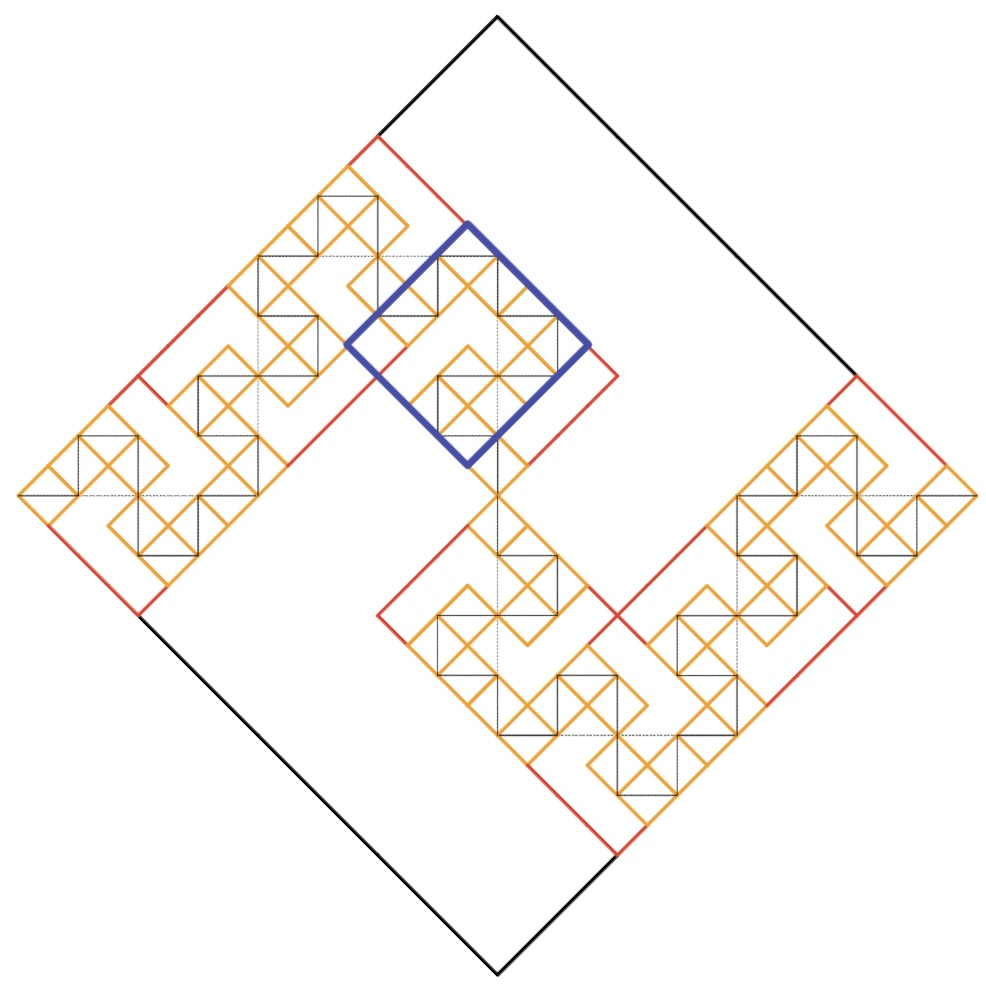
\includegraphics[scale=0.3]{solutions/section-5-0/diag-5-0-5-2.jpg}
\end{center}

It is worth mentioning why this diagram makes sense and what are the different elements of the diagram. First, note that \(M_0 = [0, 1] \subset\) the black square, which is a closed square with vertices at \((0, 0), (1, 0), \left(\frac{1}{2}, \frac{1}{2}\right), \left(\frac{1}{2}, -\frac{1}{2}\right)\). The first iteration of the black square is the eight red squares, which are all subsets of the black square. Therefore, the Minkowski Sausage \(M \subset\) the black square, and the first iteration of the Minkowski Sausage, elements in the set \(\mathcal{M}_1\), are each contained in one of the red squares. The first iteration of the red squares (the second iteration of the black square) are the orange squares, and elements in the set \(\mathcal{M}_2\) are each contained in one of the orange squares.

Now, we investigate the 10 orange squares marked in blue, and let our \(U \subset \mathcal{M}_2\) be the set of the 10 elements of \(\mathcal{M}_2\) contained in the 10 orange squares. We know that \(|\mathcal{U}| \leq |\text{blue square}| = \frac{1}{4}\) since \(\mathcal{U} \subset \) blue square.

Furthermore, each element in \(U\) has measure \(8^{-2} = \frac{1}{64}\), and therefore since there are 10 elements in \(U\), \(\mathcal{U}\) will have measure \(\frac{10}{64} = \frac{5}{32}\). Therefore,
\begin{align*}
    \h^m(M) &\leq b_2\\
    &\leq \frac{|\mathcal{U}|^m}{\mu(\mathcal{U})}\\
    &\leq \frac{4^{-\frac{3}{2}}}{\frac{5}{32}}\\
    &= \frac{\frac{1}{8}}{\frac{5}{32}}\\
    &= \frac{4}{5}\\
    &= 0.8
\end{align*}
as desired.